\section{Introduction}

This cheat sheet is intended to help with the use of the \textbf{myHOWTO} class.

The \textbf{myHOWTO} class is designed primarily for creating HOWTOs, but it can be used for any type of document if the requirements are met. 

The \textbf{myHOWTO} class is derived from the \textbf{article} class with some modifications. It uses an \textbf{A4 portrait} paper and the margin on every edge of the paper is set to \textbf{30mm}.

\qquad
\begin{myFIG}{}
	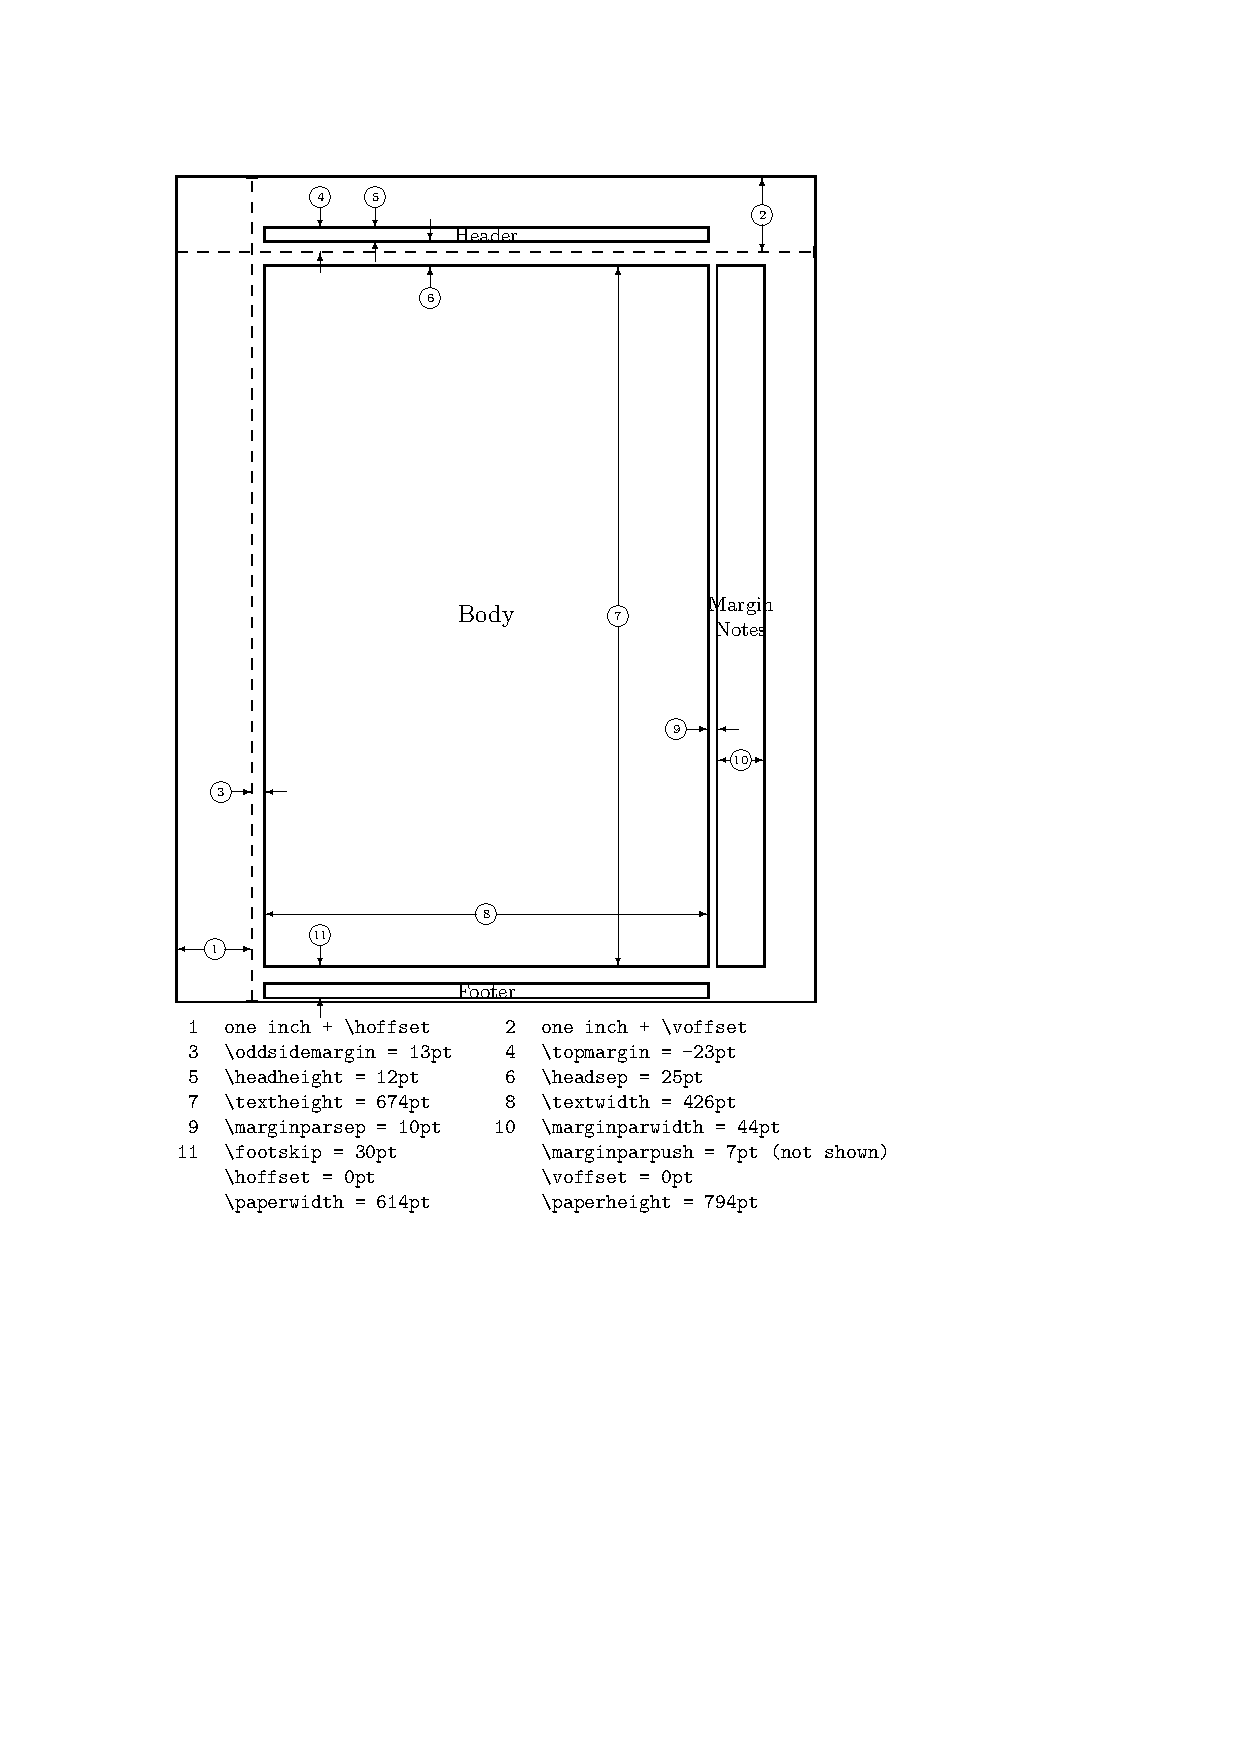
\includegraphics[page=1,scale=0.3,trim=30mm 100mm 65mm 30mm,clip]{examples/zz_bsp_file_pageLayout.pdf}
\end{myFIG}

The default font type ist \textbf{justification} and the default font size is \textbf{12pt}. The \textbf{myHOWTO} class is preconfigured with \textbf{no indentation} at the beginning of the paragraph and sets the spacing between two paragraphs to \textbf{3mm}. The header is empty, and the footer contains the current page number. Exceptions are the cover page, the table of contents, and the list of figures, where the header and footer are removed.

\qquad
\begin{myFIG}{}
	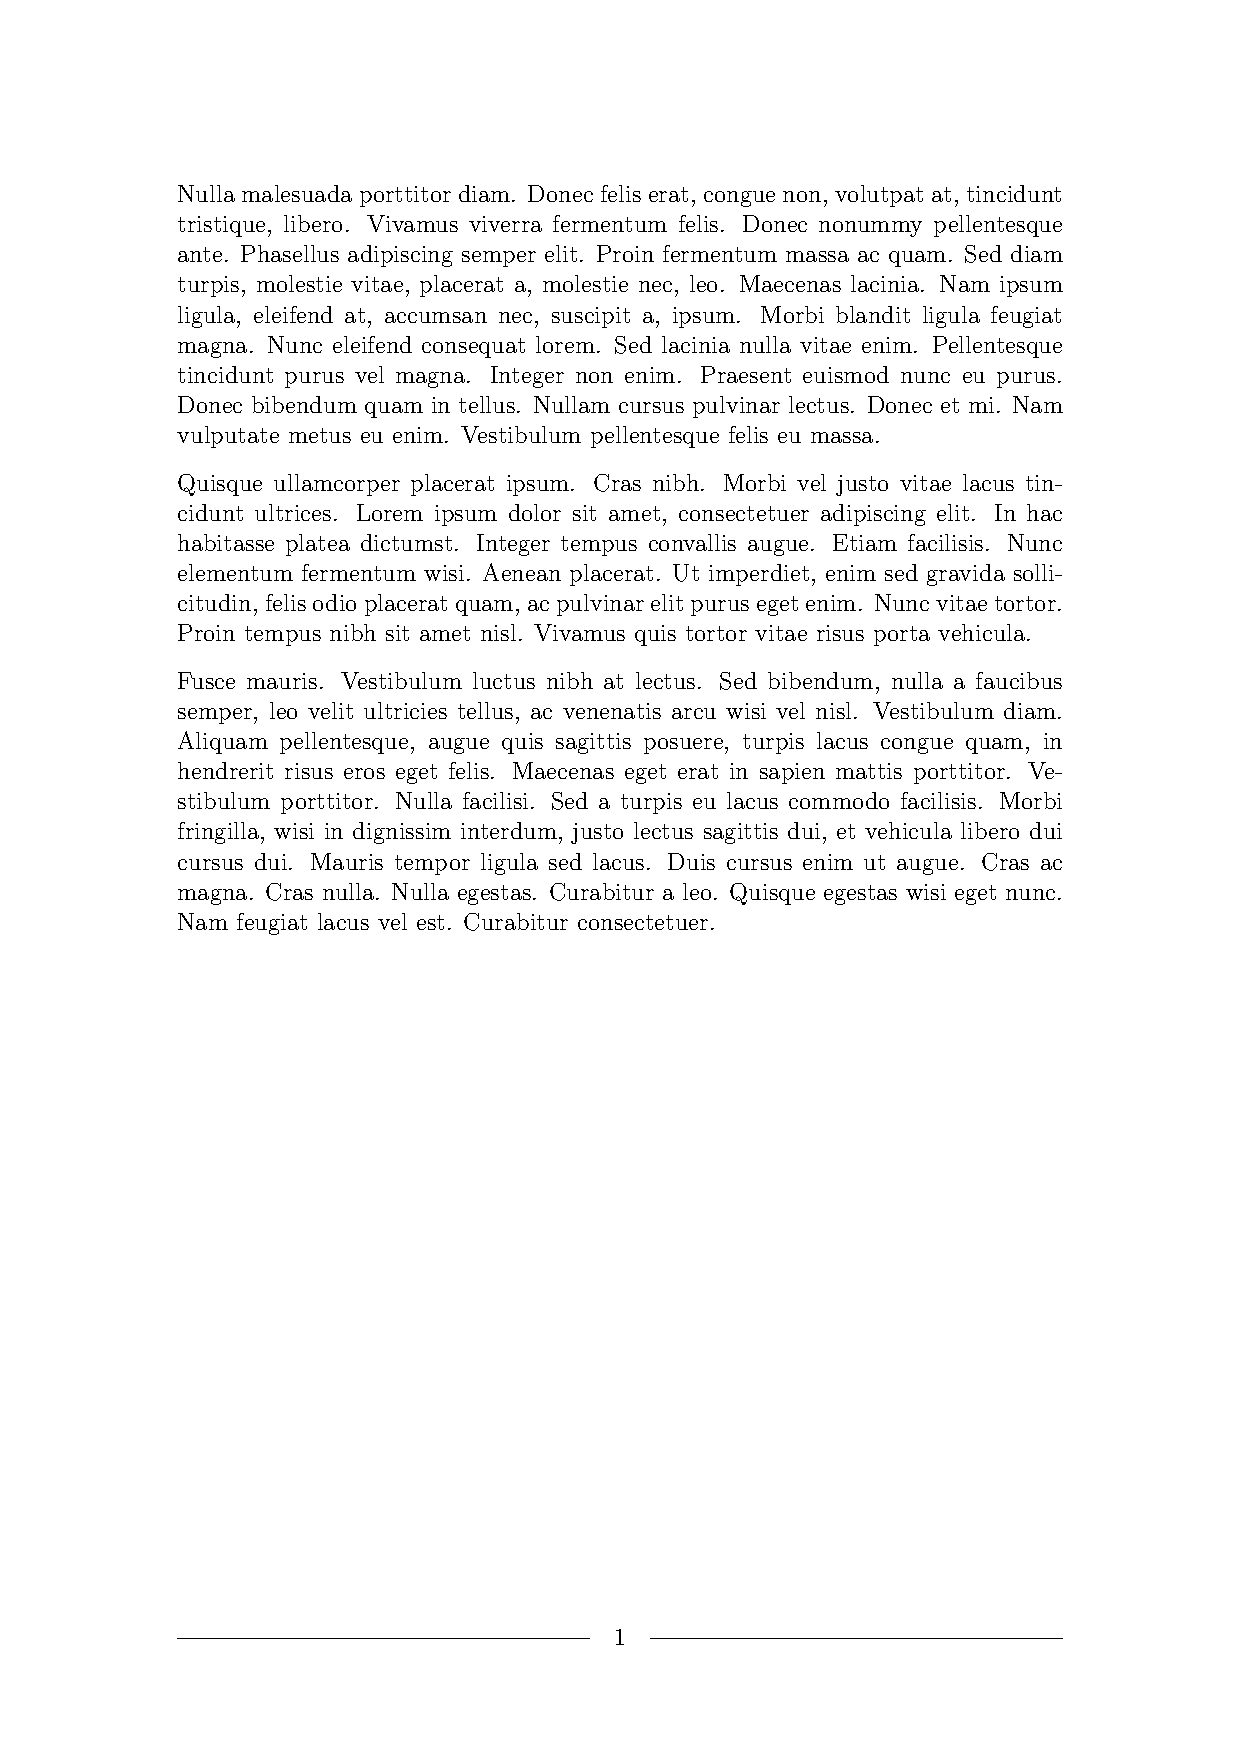
\includegraphics[page=1,scale=0.2]{examples/zz_bsp_file_parSkip.pdf}
\end{myFIG}

To use this class, it is highly recommended to have the complete \LaTeX{} distribution installed. This will avoid problems with dependencies. It is advised to use \TeX{} Live for the installation, but you can use any \LaTeX{} distribution of your choice.

The latest version of \TeX{} Live can be downloaded from \url{https://www.tug.org/}.

I personally use \TeX Studio (\url{https://www.texstudio.org/}) to write the classes \& styles and Overleaf (\url{https://github.com/overleaf/overleaf}) to write the documents. This is just a suggestion. You can use any editor of your choice.